%%%%%%%%%%%%%%%%%%%%%%%%%%%%%%%%%%%%%%%%%
% Beamer Presentation
% LaTeX Template
% Version 1.0 (10/11/12)
%
% This template has been downloaded from:
% http://www.LaTeXTemplates.com
%
% License:
% CC BY-NC-SA 3.0 (http://creativecommons.org/licenses/by-nc-sa/3.0/)
%
%%%%%%%%%%%%%%%%%%%%%%%%%%%%%%%%%%%%%%%%%

%------------------------------------------------------------------------------%
%	PACKAGES AND THEMES
%------------------------------------------------------------------------------%

\documentclass{beamer}

\mode<presentation> {

% The Beamer class comes with a number of default slide themes
% which change the colors and layouts of slides. Below this is a list
% of all the themes, uncomment each in turn to see what they look like.

%\usetheme{default}
%\usetheme{AnnArbor}
%\usetheme{Antibes}
%\usetheme{Bergen}
%\usetheme{Berkeley}
%\usetheme{Berlin}
%\usetheme{Boadilla}
%\usetheme{CambridgeUS}
%\usetheme{Copenhagen}
%\usetheme{Darmstadt}
%\usetheme{Dresden}
%\usetheme{Frankfurt}
%\usetheme{Goettingen}
%\usetheme{Hannover}
%\usetheme{Ilmenau}
%\usetheme{JuanLesPins}
%\usetheme{Luebeck}
\usetheme{Madrid}
%\usetheme{Malmoe}
%\usetheme{Marburg}
%\usetheme{Montpellier}
%\usetheme{PaloAlto}
%\usetheme{Pittsburgh}
%\usetheme{Rochester}
%\usetheme{Singapore}
%\usetheme{Szeged}
%\usetheme{Warsaw}

% As well as themes, the Beamer class has a number of color themes
% for any slide theme. Uncomment each of these in turn to see how it
% changes the colors of your current slide theme.

%\usecolortheme{albatross}
%\usecolortheme{beaver}
%\usecolortheme{beetle}
%\usecolortheme{crane}
%\usecolortheme{dolphin}
%\usecolortheme{dove}
%\usecolortheme{fly}
%\usecolortheme{lily}
%\usecolortheme{orchid}
%\usecolortheme{rose}
%\usecolortheme{seagull}
%\usecolortheme{seahorse}
%\usecolortheme{whale}
%\usecolortheme{wolverine}

% To remove the footer line in all slides, uncomment this line
%\setbeamertemplate{footline}

% To replace the footer line in all slides with a simple slide count,
% uncomment this line
%\setbeamertemplate{footline}[page number]

% To remove the navigation symbols from the bottom of all slides,
% uncomment this line
\setbeamertemplate{navigation symbols}{}
}

% Allows including images
\usepackage{graphicx}

\usepackage[utf8]{inputenc}
\usepackage{multimedia}

% Allows the use of \toprule, \midrule and \bottomrule in tables
\usepackage{booktabs}

\usepackage{duckuments}

\usepackage{aasmacros}
\usepackage[round,sort,numbers,authoryear]{natbib}
\bibliographystyle{unsrtnat}

\usepackage{wasysym}

\usepackage{cancel}

\definecolor{black}{RGB}{0,0,0}
\definecolor{thornadoblue}{HTML}{547384}
\setbeamercolor{palette primary}{bg=thornadoblue,fg=white}
%\setbeamercolor{palette secondary}{bg=black,fg=white}
%\setbeamercolor{palette tertiary}{bg=black,fg=white}
\setbeamercolor{palette quaternary}{bg=black,fg=white}
\setbeamercolor{structure}{fg=black}
\setbeamercolor{section in toc}{fg=black}
\setbeamercolor{author in head/foot}{bg=thornadoblue}
\setbeamercolor{title in head/foot}{bg=black}
\usepackage[font={color=black},figurename=Figure,bf]{caption}
\setbeamercolor{normal text}{fg=black}

\usefonttheme[onlymath]{serif}

% https://tex.stackexchange.com/questions/33969/changing-font-size-of-selected-slides-in-beamer
\newcommand\Fontvi{\fontsize{8}{8.2}\selectfont}

% Aliases
\newcommand{\thornado}{\texttt{thornado}}
\newcommand{\poseidon}{Poseidon}
\newcommand{\amrex}{AMReX}
\newcommand{\ul}{\underline}


% --- TITLE PAGE SLIDE ---

\title[NR Community Call]{\thornado-Hydro (xCFC)}

\author{Samuel J. Dunham}
\date{October 2, 2023}

\begin{document}

\begin{frame}

  \titlepage

  \begin{center}
    Brandon Barker (MSU/LANL), %
    Jesse Buffaloe (UTK), \\
    SJD (Vanderbilt,UTK), %
    Eirik Endeve (ORNL/UTK), \\
    Anthony Mezzacappa (UTK), %
    Nick Roberts (UTK)
  \end{center}

  \vspace{-1em}

  \begin{columns}[c]

    \column{.3\textwidth}
      \begin{center}\thornado\end{center}
      \vspace{-1.5em}
      \begin{figure}[htb!]
        \centering
        
\includegraphics[width=0.5\textwidth]{fig.thornado.png}
      \end{figure}

    \column{.3\textwidth}
      \begin{center}My Website\end{center}
      \vspace{-1.5em}
      \begin{figure}[htb!]
        \centering
        
\includegraphics[width=0.5\textwidth]{fig.website.png}
      \end{figure}

  \end{columns}

\end{frame}

\begin{frame}

  \begin{figure}[ht]
    \centering
    
\includegraphics[width=0.3\textwidth]{fig.thornado_logo.png}
  \end{figure}

  \begin{center}

    \ul{t}oolkit for
    \ul{h}igh-\ul{or}der
    \ul{n}eutrino-r\ul{ad}iation hydr\ul{o}dynamics\\[1em]

    \begin{columns}[c]

      \column{0.5\textwidth}

        \begin{itemize}
          \item
            DG
          \item
            SSPRK/IMEX
          \item
            GR (xCFC)
          \item
            Hydro (Valencia)
          \item
            Neutrino transport (M1)
          \item
            Interfaces to tabulated EoS/Opacities
            (weaklib: \url{https://github.com/starkiller-astro/weaklib})
        \end{itemize}

      \column{0.5\textwidth}

        \begin{itemize}
          \item
            Fluid self-gravity via \poseidon:
            \url{https://github.com/jrober50/Poseidon}
          \item
            GPUs via OpenACC and OpenMP pragmas
          \item
            MPI parallelism via \amrex
          \item
            AMR via \amrex
        \end{itemize}

    \end{columns}

  \end{center}

\end{frame}

\begin{frame}
\frametitle{Discontinuous Galerkin (DG)}

  \vspace{-1em}

  \begin{equation*}
    u_{h}\left(x,y,t\right)
    :=\sum\limits_{i=1}^{N}\sum\limits_{j=1}^{N}
      u_{i,j}\left(t\right)\,\ell_{i}\left(x\right)\,\ell_{j}\left(y\right)
  \end{equation*}

  \begin{figure}[htb!]
    \centering
    \begin{minipage}{0.28\textwidth}
      \includegraphics[width=\textwidth]%
      {fig.DG_2D_N2.png}
    \end{minipage}
    \hfill
    \begin{minipage}{0.28\textwidth}
      \includegraphics[width=\textwidth]%
      {fig.DG_2D_N3.png}
    \end{minipage}
    \hfill
    \begin{minipage}{0.3\textwidth}
      \includegraphics[width=\textwidth]%
      {fig.DG_2D_Exact.png}
    \end{minipage}
    \hfill
  \end{figure}

\end{frame}

\begin{frame}

  \begin{figure}[htb!]
    \centering
    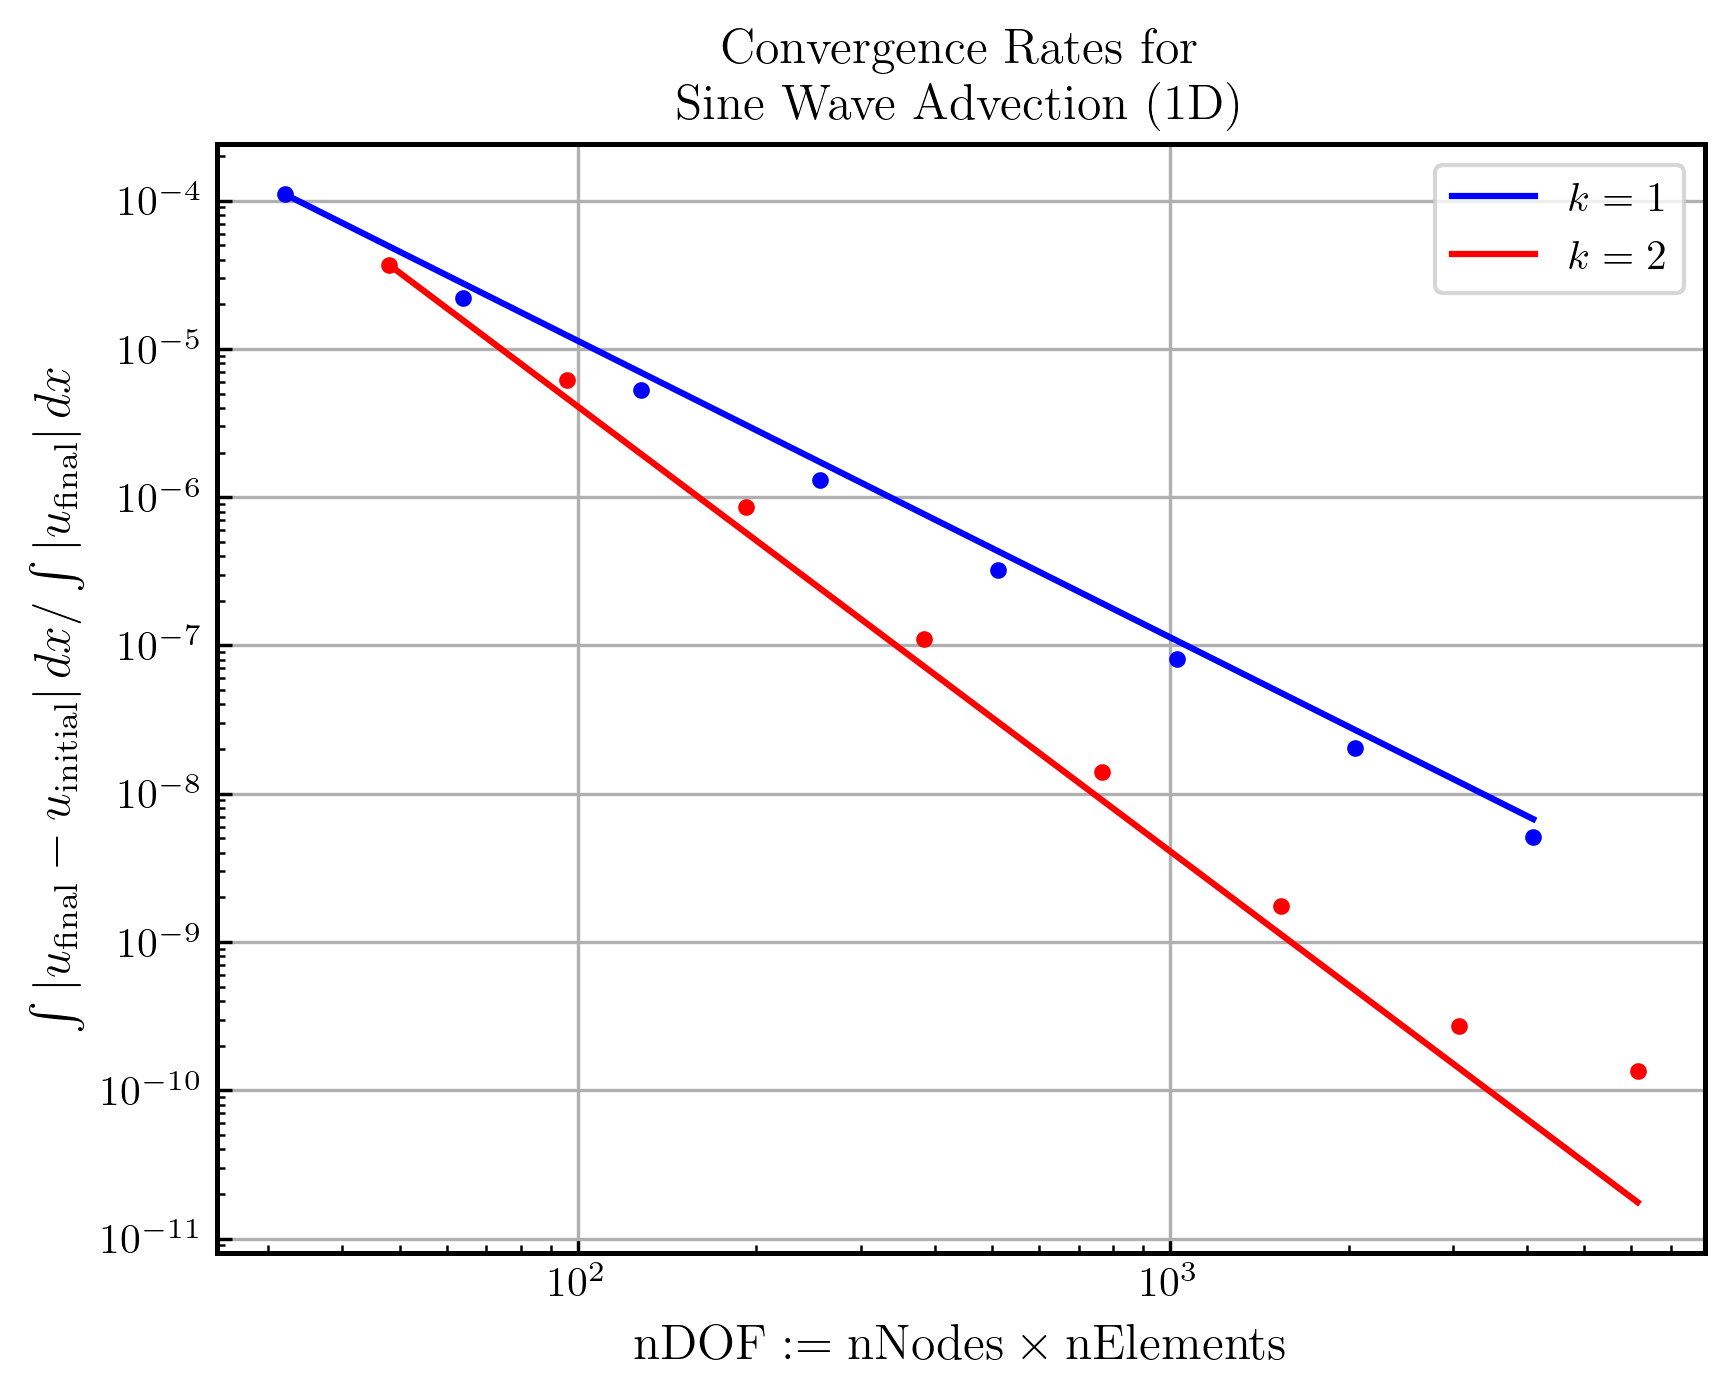
\includegraphics[width=0.8\textwidth]{fig.ConvergenceRates.png}
  \end{figure}

\end{frame}

\begin{frame}

  \begin{figure}[htb!]
    \centering
    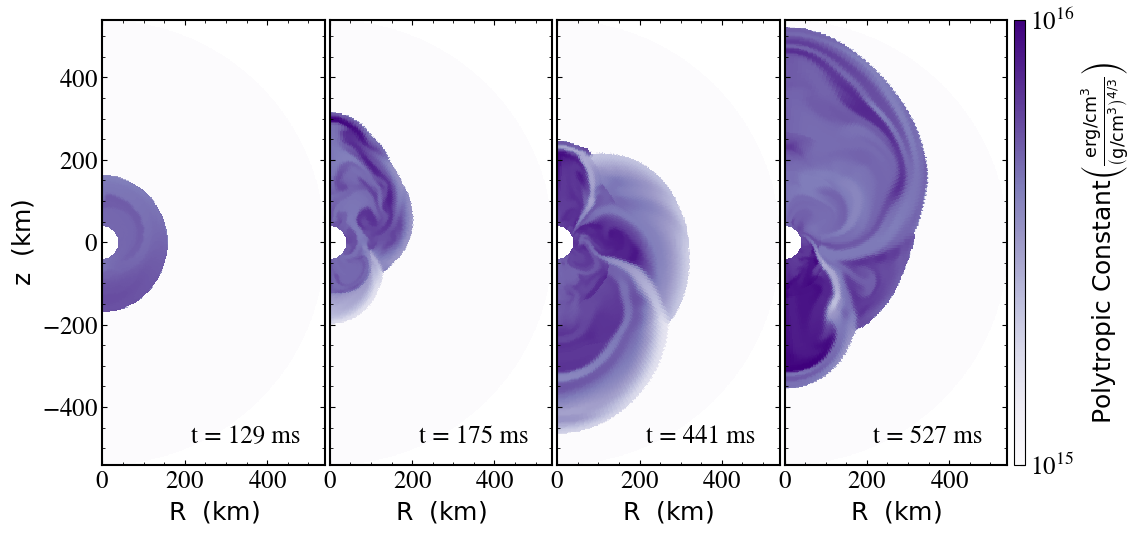
\includegraphics[width=0.9\textwidth]{fig.sasi.png}
  \end{figure}

\end{frame}

\begin{frame}

  \begin{figure}[htb!]
    \centering
    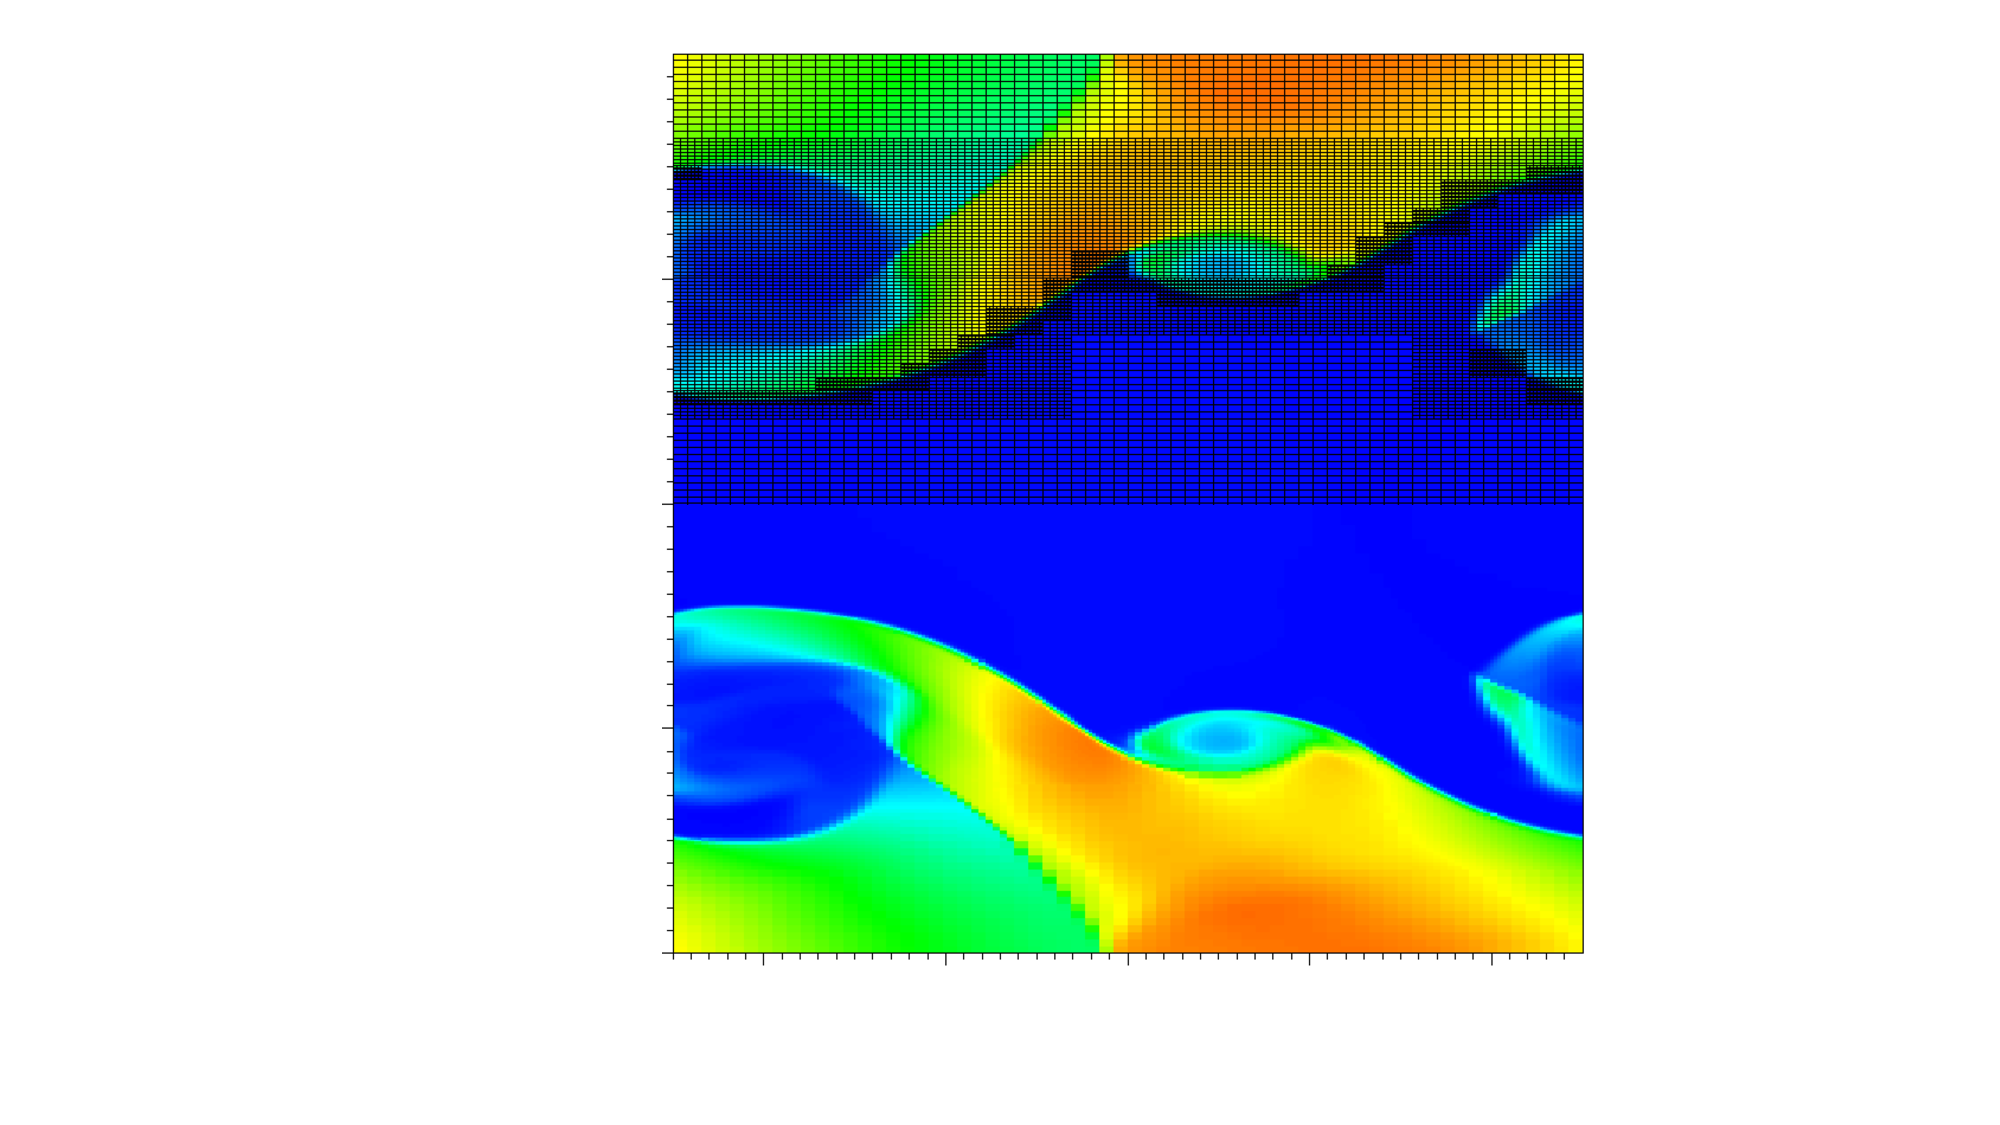
\includegraphics[width=0.7\textwidth]{fig.KHI.pdf}
  \end{figure}

\end{frame}

\begin{frame}

  \begin{figure}[htb!]
    \centering
    \begin{minipage}{0.49\textwidth}
      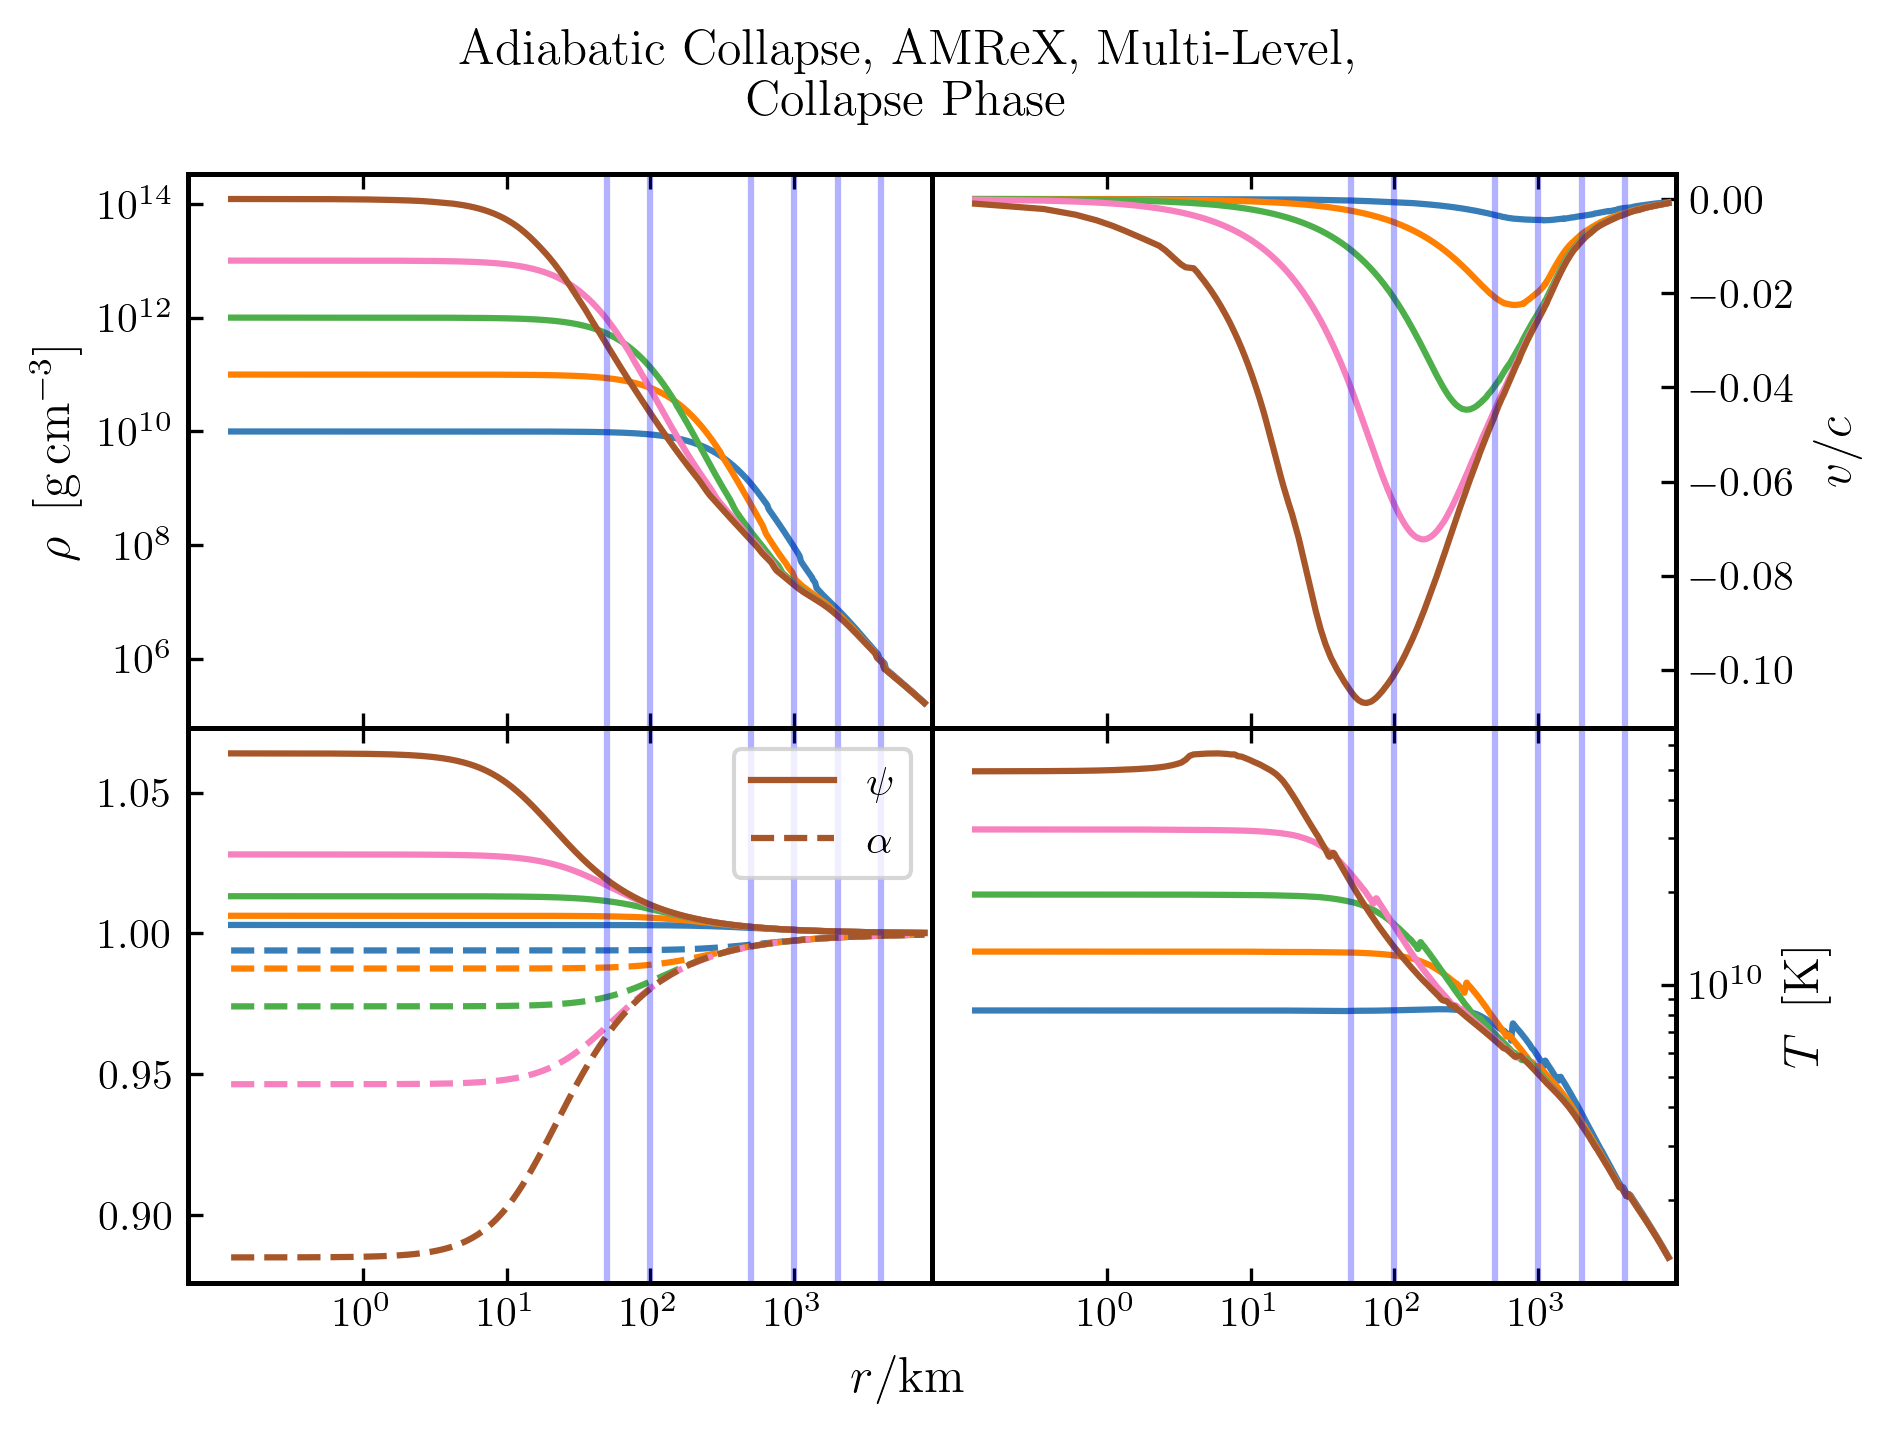
\includegraphics[width=\textwidth]{fig.Collapse.png}
    \end{minipage}
    \begin{minipage}{0.49\textwidth}
      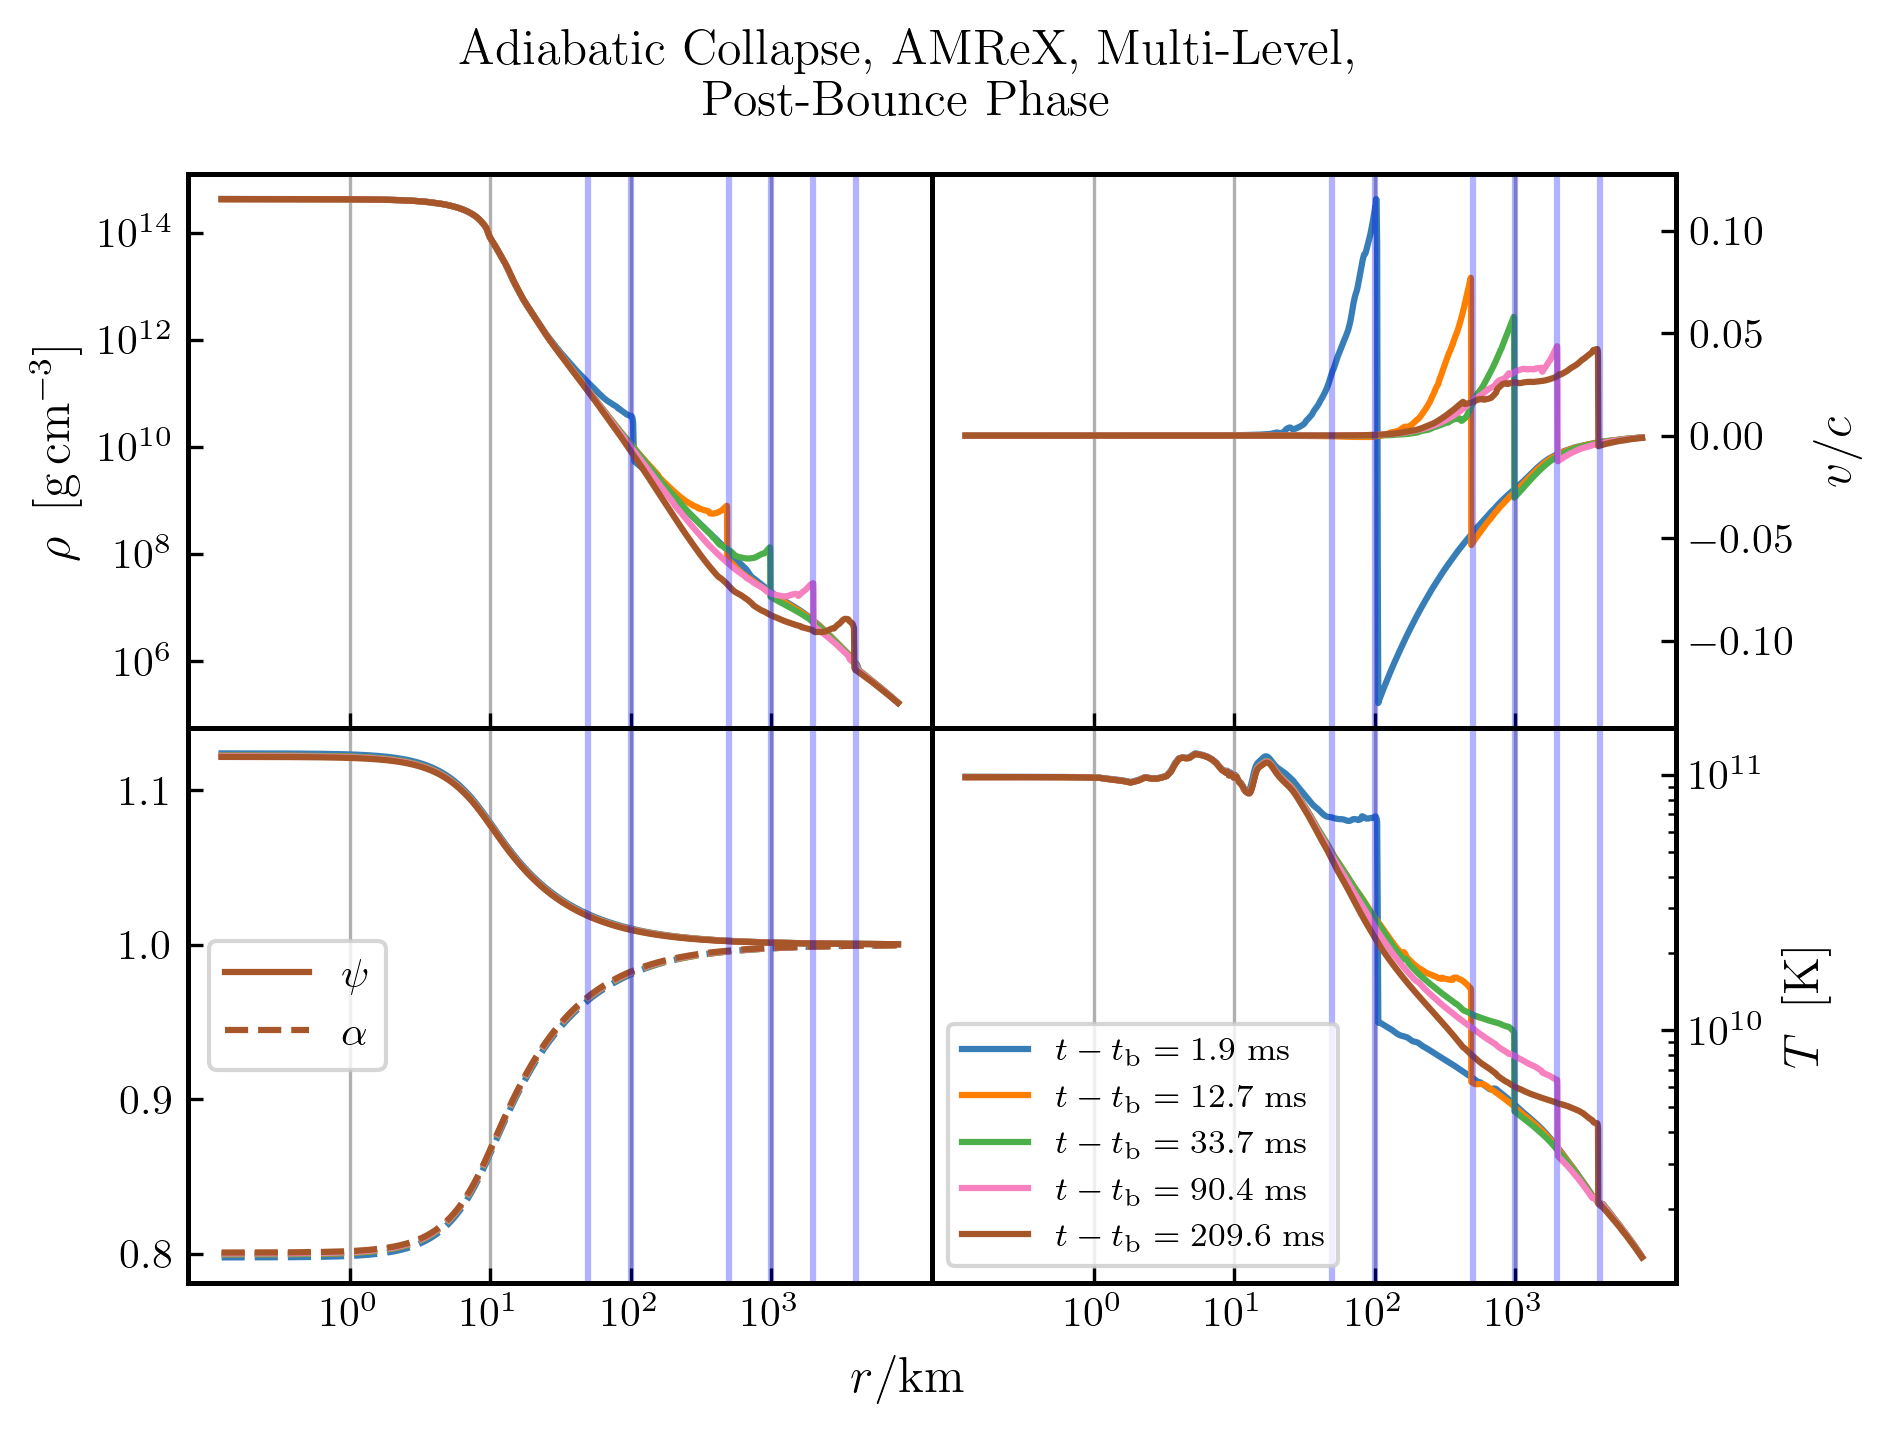
\includegraphics[width=\textwidth]{fig.PostBounce.png}
    \end{minipage}
  \end{figure}

\end{frame}

\end{document}
%------------------------------------------------------------------------------%
